% Preface this by describing what you have with you today.
\begin{frame}{Qu'est-ce que vous avez? \gloss{What do y'all have?}}
  \small
  En groupes de 3 ou 4, demandez à votre tour ce que les autres ont aujourd'hui, puis comparez si vous avez les mêmes choses ou non. \\
  \tinygloss{In groups of 3 or 4, take turns asking each other what each of you have with you today, then compare if you have the same things or not.
  For example:}
  \begin{columns}
    \column{0.6\textwidth}
      \begin{itemize}
        \item[E1:] (to E2) Qu'est-ce que tu as?
        \item[] \tinygloss{What do you have?}
        \item[E2:] J'ai un \alert{stylo}, un ordinateur et des feuilles de papier.
        \item[] \tinygloss{I have a \alert{pen}, a computer et some pieces of paper.}
        \item[E2:] (to E3) Qu'est-ce que tu as?
        \item[] \tinygloss{What do you have?}
        \item[E3:] J'ai un cahier, un crayon et un \alert{stylo}. Nous avons \alert{des stylos}.
        \item[] \tinygloss{I have a notebook, a pencil and a \alert{pen.} We have \alert{pens}.}
      \end{itemize}
    \column{0.4\textwidth}
      \begin{center}
        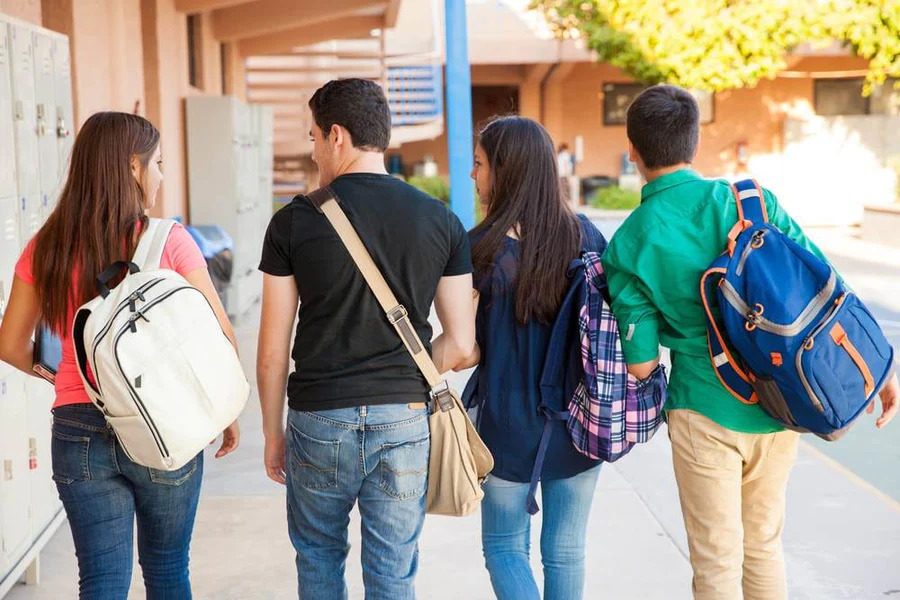
\includegraphics[scale=0.15]{sacs.jpg}
      \end{center}
  \end{columns}
\end{frame}